% Document class
\documentclass[11pt]{article}

% Import packages
% Packages: General typesetting
\usepackage{graphicx} % Include graphics
\usepackage{float} % Helps with typesetting figures
\usepackage[export]{adjustbox} % Helps with typesetting figures
\usepackage{fancyhdr} % Headers and footers

% Packages: Environments
\usepackage{amsmath} % Equation, align environments
\usepackage{amsthm} % Typesetting theorems and proofs
\usepackage{enumerate} % List / enumerations

% Packages: Maths
\usepackage{amssymb} % A bunch of symbols
\usepackage{esint} % Integration symbols
\usepackage{cancel} % Cancelling mathematical terms
\usepackage{braket} % Braket notation

% Packages: Miscellaneous
\usepackage{hyperref}
\hypersetup{
    colorlinks=false,
    pdfborder={0 0 0},
}
\usepackage{custom_macros}

\pagestyle{fancy}

% Can you suppress the first running heading?

\begin{document}
\vspace{-2cm}
\begin{center}
    % Subject name
    {\Large\bf Torque of Concentric Elliptic Rings} \\
    \vspace{5mm}
    %\vspace{-3cm}
    {\Large Pavadol Yamsiri} \\
    \vspace{3mm}
    Supervisors: Joss Bland-Hawthorn, Thor Tepper-Garcia \\
    \vspace{2mm}
    Sydney Institute for Astronomy
\end{center}
\vspace{0.5mm}

% TODO: Add bibtex references
\begin{abstract}
    % find earliest ref. to this - probably first ever discussion of spiral arms or soon after.
    Astronomers have long known that they can produce spiral perturbations in a disc by using concentric elliptic annuli
    (or rings) that are rotated as a slow function of the ellipse's major axis position angle (Lindblad 1956). To our knowledge,
    this idea has only ever been explored geometrically (e.g. Kalnajs 1973) and never used as a toy model involving kinematic or
    dynamic arguments. Inspired by recent N-body simulations of an impulse-driven density wave in a cold stellar disc, we
    investigate the nature of that wave. With the aid of a fully dynamical toy model in 2D and 3D, we see that the early spiral
    wave (seen to wrap up as time passes) is entirely kinematic, with no forces acting. The initial impulse perturbs the disc
    such that the low-order vertical and radial frequencies are simple perturbations of the disc potential. In the plane, this
    gives rise to coherent rotation of the ellipses (see above) following Lindblad's formula \( \Omega(R)-\kappa(R)/2 \) where
    \( \Omega \) is the angular frequency of an ellipse's major axis, and \( \kappa \) is the radial frequency. But at late times,
    the wrapping stalls and the kinematic wave loses its coherence. At this point, the spiral arms become a dynamical density
    wave, where the inter-arm forces lead to instability, as seen in the simulations. We see this behaviour in both gas-free and
    gas-rich simulated discs (Bland-Hawthorn \& Tepper-Garcia 2021; Tepper-Garcia et al 2022).
\end{abstract}

\section{The Potential of an Elliptic Ring}

\begin{figure}[h!]
    \begin{center}
        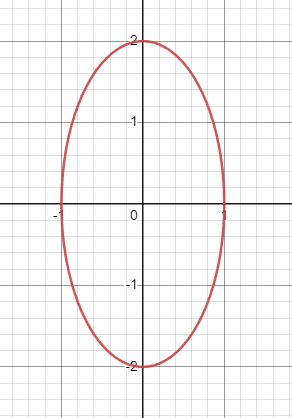
\includegraphics[scale=0.5]{resources/elliptic_ring.png}
        \caption{An elliptic ring.}
        \label{potential::elliptic_ring}
    \end{center}
\end{figure}

Consider an elliptic ring (see Figure~\ref{potential::elliptic_ring}) with
\begin{equation}
    \mu = \frac{M}{L}
\end{equation}
where \( \mu \) is the mass per unit length, \( M \) is the total mass of the ring and \( L \) is the perimeter of the ring.

The potential of a small segment of the ring is given by the equation
\begin{equation}
    \delta \Phi(\vec{r}) = -\frac{Gm_{\text{segment}}}{\left|\vec{r} - \vec{r}_{\text{segment}}\right|}
\end{equation}
The mass of the segment is
\begin{equation}
    m_{\text{segment}} = \mu \delta s
\end{equation}
where \( \delta s \) is the length of the small segment of the ellipse, so
\begin{equation}
    \delta \Phi(\vec{r}) = -\frac{G\mu \delta s}{\left|\vec{r} - \vec{r}_{\text{segment}}\right|}
\end{equation}
Therefore, the potential of the entire elliptic ring is simply
\begin{equation}
    \Phi_{\text{ring}}(\vec{r}) = G\mu \int \frac{\mathrm{d}s}{\left|\vec{r} - \vec{r}_{\text{segment}}\right|}
\end{equation}
In order to integrate, we will need to express the line element in coordinates that lie on the ellipse.
The Cartesian coordinates \( (x, y) \) of a point on the ellipse can be written as
\begin{align}
    x & = aR\cos{\theta} \\
    y & = bR\sin{\theta}
\end{align}
where \( a \) and \( b \) are the scale width and height of the ellipse respectively, \( R \) is the scale length and \( \theta \)
is a parameter that varies from \( 0 \) to \( 2\pi \). We want to get the differentials of these coordinates in terms of
\( d\theta \) to aid in the integration.
\begin{align}
    \mathrm{d}x & = -aR\sin{\theta} \mathrm{d}\theta \\
    \mathrm{d}y & = bR\cos{\theta} \mathrm{d}\theta
\end{align}
The line element \( \mathrm{d}s \) is hence given by
\begin{align}
    {\mathrm{d}s}^{2}    & = {\mathrm{d}x}^{2} + {\mathrm{d}y}^{2} \nonumber                                                      \\
                         & = a^2R^2\sin^2{\theta} {\mathrm{d}\theta}^2 + b^2R^2\cos^2{\theta} {\mathrm{d}\theta}^2 \nonumber      \\
                         & = R^2\left(a^2\sin^2{\theta} + b^2\cos^2{\theta}\right) {\mathrm{d}\theta}^2 \nonumber                 \\
                         & = R^2\left(a^2\left(1 - \cos^2{\theta}\right)+ b^2\cos^2{\theta}\right) {\mathrm{d}\theta}^2 \nonumber \\
                         & = R^2\left(a^2 - (a^2 - b^2)\cos^2{\theta}\right) {\mathrm{d}\theta}^2 \nonumber                       \\
                         & = a^2R^2\left(1 - \left(1 - \frac{b^2}{a^2}\right)\cos^2{\theta}\right) {\mathrm{d}\theta}^2 \nonumber \\
                         & = a^2R^2 \left(1 - e^2\cos^2{\theta}\right) {\mathrm{d}\theta}^2 \nonumber                             \\
    \implies \mathrm{d}s & = aR\sqrt{1 - e^2\cos^2{\theta}} \mathrm{d}\theta
\end{align}
where \( e \) is the eccentricity of the ellipse equal to \( e = \sqrt{1 - \frac{b^2}{a^2}} \).
Finally, the potential \( \Phi_{\text{ring}}(\vec{r}) \) evaluated at \( \vec{r} \) is given by the integral
\begin{equation}
    \Phi_{\text{ring}}(\vec{r}) = -G \mu a R \int_{0}^{2\pi} \frac{\sqrt{1 - e^2\cos^2{\theta}}}{\left|\vec{r} - \vec{r}_{\text{ellipse}}\right|} \,\,{} \mathrm{d}\theta
\end{equation}
The potential in terms of Cartesian coordinates \( (x, y) \) can be written as
\begin{equation}
    \Phi_{\text{ring}}(x, y) = -G \mu R \int_{0}^{2\pi} \frac{\sqrt{1 - e^2\cos^2{\theta}}}{\sqrt{{(x - x_{\text{ellipse}})}^{2} + {(y - y_{\text{ellipse}})}^{2}}} \,\,{} \mathrm{d}\theta
\end{equation}
Substituting in for \( x \) and \( y \) their parametric forms we obtain
\begin{equation}
    \Phi_{\text{ring}}(x, y) = -G \mu a R \int_{0}^{2\pi} \frac{\sqrt{1 - e^2\cos^2{\theta}}}{\sqrt{{(x - aR\cos{\theta})}^{2} + {(y - bR\sin{\theta})}^{2}}} \,\,{} \mathrm{d}\theta
\end{equation}
This only applies for ellipses coaxial with the Cartesian coordinate axes, so in order to get the potential of a rotated ellipse,
we want the coordinates of the ellipse rotated by an angle \( \alpha \), say anti-clockwise
\begin{align}
    \begin{pmatrix}
        x' \\ y'
    \end{pmatrix} & = \begin{pmatrix}
                          \cos{\alpha} & -\sin{\alpha} \\
                          \sin{\alpha} & \cos{\alpha}
                      \end{pmatrix} \begin{pmatrix}
                                        x \\ y
                                    \end{pmatrix}                              \\
                    & = \begin{pmatrix}
                            \cos{\alpha} & -\sin{\alpha} \\
                            \sin{\alpha} & \cos{\alpha}
                        \end{pmatrix} \begin{pmatrix}
                                          aR\cos{\theta} \\ bR\sin{\theta}
                                      \end{pmatrix} \nonumber             \\
    \begin{pmatrix}
        x' \\ y'
    \end{pmatrix} & = R\begin{pmatrix}
                           a\cos{\alpha}\cos{\theta} - b\sin{\alpha}\sin{\theta} \\
                           a\sin{\alpha}\cos{\theta} + b\cos{\alpha}\sin{\theta}
                       \end{pmatrix} \label{potential::rotated_ellipse_cartesian}
\end{align}
% TODO: I don't know if this is correct. theta is the angle of the ellipse, not the angle of rotation, so the line element might
% not be the same.
So the potential of a rotated elliptic ring is
\begin{equation}
    \Phi_{\text{ring}}(x, y) = -G \mu a R \int_{0}^{2\pi} \frac{\sqrt{1 - e^2\cos^2{\theta}}}{\sqrt{{(x - x')}^{2} + {(y - y')}^{2}}} \,\,{} \mathrm{d}\theta
\end{equation}
where \( (x', y') \) are given by Equation~\ref{potential::rotated_ellipse_cartesian}.
\newpage
\section{The Torque from an Elliptic Ring}
The torque imparted by a force \( \vec{F} \) on a point mass at \( \vec{r} \) is given by
\begin{equation}
    \vec{\tau} = \vec{r} \times \vec{F}
\end{equation}
The gravitational force on a mass \( m \) at \( \vec{r} \) exerted by a gravitational potential \( \Phi \) is given by
\begin{equation}
    \vec{F}(\vec{r}) = -m\vec{\nabla} \Phi(\vec{r})
\end{equation}
so we have that the torque is equal to
\begin{equation}
    \vec{\tau} = -m\vec{r} \times \vec{\nabla} \Phi(\vec{r})
\end{equation}
Lets say we have another elliptic ring centred at the origin and with the same eccentricity,
with radius \( R_2 \) and rotated by an angle \( \alpha \) anti-clockwise. The torque
imparted by the first elliptic ring onto the second elliptic ring can be calculated by
first considering the torque on a line segment of the second elliptic ring
\begin{equation}
    \delta \tau = -\nu \vec{r} \times \vec{\nabla} \Phi(\vec{r}) \delta s
\end{equation}
where \( \nu = \frac{m}{l} \) is the mass per unit length of the second elliptic ring, \( M \) is the
total mass of the second elliptic ring and \( L \) is the perimeter of the second elliptic ring. The total
torque is then just the integral over the entire ring
\begin{equation}
    \tau
    = -\nu \int \vec{r} \times \vec{\nabla} \Phi(\vec{r}) \,{}\,{} \mathrm{d}s
    = -a\nu R \int_{0}^{2\pi} \sqrt{1 - e^2\cos^2{\theta}} \left(\vec{r} \times \vec{\nabla} \Phi(\vec{r})\right) \,\,{} \mathrm{d}\phi
\end{equation}
These integrals do not have closed form solutions and so can only be solved via numerical methods.

\subsection{Particle Approximation}
One method to approximate the torque on the second ring, is to approximate the ring by
dividing it into a \( N \) point particles uniformly distributed around the
ring\footnote{The distance between each point on the ellipse is the same arc length.}.
The torque exerted by the first elliptic ring
only\footnote{There are no forces between particles part of the same elliptic ring, as the rings are rigid}
is calculated for all \( N \) particles, and then total torque is simply the sum of the
torques on the \( N \) particles.
\begin{equation}
    \tau \approx \sum_{n=1}^{N} \tau_n = \frac{M}{N} \sum_{n=1}^{N} \vec{r_n} \times \vec{\nabla} \Phi(\vec{r_n})
\end{equation}
The masses of the particles is \( M_n = \frac{M}{N} \) where \( M \) is the total mass of the second elliptic ring and \( N \) is
number of particles.

\subsection{Results}
Let there be two elliptic rings with equal masses \( 1000 \),
radii \( R_1 = 1 \) and \( R_2 = 3 \) and axes ratio \( \frac{b}{a} = 2 \).
We will rotate the second elliptic ring for a full revolution and calculate the torque along the
\( z \)-axis on the second elliptic ring by exerted by the first elliptic ring and vice versa.

\begin{figure}[h!]
    \begin{center}
        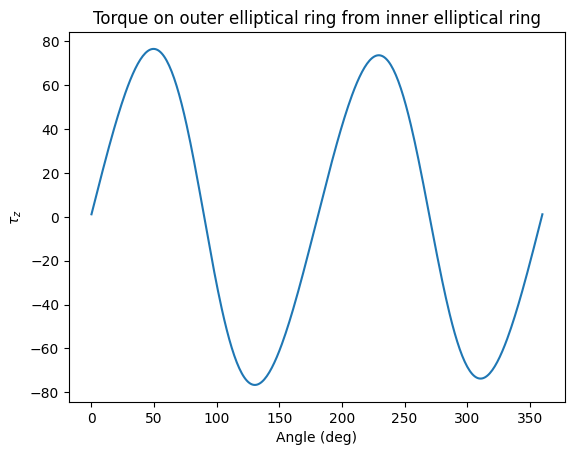
\includegraphics[scale=0.9]{resources/torque_on_outer_ellipse.png}
        \caption{Torque exerted by inner elliptic ring on outer elliptic ring.}
        \label{results::inner_on_outer}
    \end{center}
\end{figure}

It is clear that the torque is greatest when the phase difference is \( \pi / 4 \), and zero
when the phase difference is \( 0 \) or \( \pi / 2 \).
\newpage
\section{Equations of Motion}
Currently we only have the torque exerted on a ring. In order to obtain the equations of motion governing the orientation of the
ring, we need the relationship between torque and angular acceleration. Torque is defined as
\begin{equation}
    \vec{\tau} = \dbyd{\vec{L}}{t}\label{eq:torque_angular_momentum}
\end{equation}
the time derivative of the angular momentum \( \vec{L} \) which itself is given by
\begin{equation}
    \vec{L} = \mathbf{I} \vec{\omega}\label{eq:angular_momentum}
\end{equation}
where \( \mathbf{I} \) is the called the inertia tensor and \( \vec{\omega} \) is the angular velocity vector.
Substituting Eqn.~\ref{eq:angular_momentum} into
Eqn.~\ref{eq:torque_angular_momentum} gives
\begin{align}
    \vec{\tau} & = \dbyd{}{t} \left(\mathbf{I} \vec{\omega}\right) \nonumber                                                 \\
               & = \dbyd{\mathbf{I}}{t} \vec{\omega} + \mathbf{I} \dbyd{\vec{\omega}}{t} \nonumber                           \\
               & = \dbyd{\mathbf{I}}{t} \vec{\omega} + \mathbf{I} \vec{\alpha} \label{eq:torque_angular_momentum_expression}
\end{align}
where \( \vec{\alpha} \) is the angular acceleration vector. In order to get an expression for the term \( \dbyd{\mathbf{I}}{t} \),
we can express the inertia tensor as being a rotation of a constant inertia tensor \( \tilde{\mathbf{I}} \) calculated in a fixed
inertial frame of the ring
\begin{equation}
    \mathbf{I} = \mathbf{R} \tilde{\mathbf{I}} {\mathbf{R}}^{T}
\end{equation}
where \( \mathbf{R} \) is the rotation matrix that transform from the fixed inertial frame to our current frame. Taking the time
derivative of this expression gives
\begin{align}
    \dbyd{\mathbf{I}}{t} =
    \dbyd{\mathbf{R}}{t} \tilde{\mathbf{I}} {\mathbf{R}}^{T}
    + \mathbf{R} \tilde{\mathbf{I}} \dbyd{{\mathbf{R}}^{T}}{t} \label{eq:inertia_tensor_time_derivative}
\end{align}
The time derivative of the rotation matrix can be written in terms of the angular velocity \( \vec{\omega} \)
\begin{equation}
    \dbyd{\mathbf{R}}{t} = {\mathbf{\omega}}_{\times} \mathbf{R} \label{eq:rotation_matrix_time_derivative}
\end{equation}
where \( {\mathbf{\omega}}_{\times} \) is a skew-symmetric matrix defined as the map \( \vec{x} \mapsto \vec{\omega} \times \vec{x} \),
i.e.~matrix representation of the cross product with \( \vec{\omega} \). The components are
\begin{equation}
    {\mathbf{\omega}}_{\times} = \begin{pmatrix}
        0         & -\omega_z & \omega_y  \\
        \omega_z  & 0         & -\omega_x \\
        -\omega_y & \omega_x  & 0
    \end{pmatrix}
\end{equation}
Substituting Eqn.~\ref{eq:rotation_matrix_time_derivative} into Eqn.~\ref{eq:inertia_tensor_time_derivative} gives
\begin{align}
    \dbyd{\mathbf{I}}{t}
     & = \dbyd{\mathbf{R}}{t} \tilde{\mathbf{I}} {\mathbf{R}}^{T}
    + \mathbf{R} \tilde{\mathbf{I}} {\left(\dbyd{\mathbf{R}}{t}\right)}^{T} \nonumber                               \\
     & = \left({\mathbf{\omega}}_{\times} \mathbf{R}\right) \tilde{\mathbf{I}} {\mathbf{R}}^{T}
    + \mathbf{R} \tilde{\mathbf{I}} {\left({\mathbf{\omega}}_{\times} \mathbf{R}\right)}^{T} \nonumber              \\
     & = {\mathbf{\omega}}_{\times} \left(\mathbf{R}\tilde{\mathbf{I}}{\mathbf{R}}^{T}\right)
    + \mathbf{R} \tilde{\mathbf{I}} {\left({\mathbf{R}}^{T} {\mathbf{\omega}_{\times}}^{T}\right)} \nonumber        \\
     & = {\mathbf{\omega}}_{\times} \mathbf{I}
    + \left(\mathbf{R} \tilde{\mathbf{I}} {\mathbf{R}}^{T} \right) \left(-\mathbf{\omega}_{\times}\right) \nonumber \\
    \implies \dbyd{\mathbf{I}}{t}
     & = {\mathbf{\omega}}_{\times} \mathbf{I}
    - \mathbf{I}{\mathbf{\omega}}_{\times} \label{eq:inertia_tensor_time_derivative_expression}
\end{align}
Using the Eqn.~\ref{eq:inertia_tensor_time_derivative_expression} in Eqn.~\ref{eq:torque_angular_momentum_expression} gets
\begin{align}
    \vec{\tau}          & = \left({\mathbf{\omega}}_{\times} \mathbf{I} - \mathbf{I}{\mathbf{\omega}}_{\times}\right) \vec{\omega}
    + \mathbf{I} \vec{\alpha} \nonumber                                                                                            \\
                        & = {\mathbf{\omega}}_{\times} \mathbf{I} \vec{\omega} - \mathbf{I}{\mathbf{\omega}}_{\times} \vec{\omega}
    + \mathbf{I} \vec{\alpha} \nonumber                                                                                            \\
                        & = {\mathbf{\omega}}_{\times} \vec{L} - \mathbf{I}\left(\vec{\omega} \times \vec{\omega}\right)
    + \mathbf{I} \vec{\alpha} \nonumber                                                                                            \\
    \implies \vec{\tau} & = \vec{\omega} \times \vec{L} + \mathbf{I} \vec{\alpha}
\end{align}
Now rearrange to get an expression for the angular acceleration
\begin{equation}
    \dbyd{\vec{\omega}}{t} = \vec{\alpha}
    = {\mathbf{I}}^{-1} \left(\vec{\tau} - \vec{\omega} \times \vec{L}\right)
        = {\mathbf{I}}^{-1} \left[\vec{\tau} - \vec{\omega} \times \left(\mathbf{I} \times \vec{\omega}\right)\right]
\end{equation}
Currently, we are missing the differentual equation for the orientation of the ring. This is not such a simple task as
integrating the angular velocity with respect to time due to the intricacies of rotations in 3D space. See
Section~\ref{sec:quaternions} to see how angular velocity will be integrated.

\subsection{Inertia Tensor}
In this section we will derive inertia tensor of an elliptic ring about its centre of mass in the ring's frame of reference.
In this frame of reference, the ring lies on the \( x-y \)-plane and the \( z \)-axis is perpendicular to the plane of the ring.
The \( x \)-axis will be taken to be the major axis of the ellipse and the \( y \)-axis will be taken to be the minor axis of the
ellipse.

The inertia tensor is a rank 2 symmetric tensor which can be written in matrix form as
\begin{equation}
    \mathbf{I} = \begin{pmatrix}
        I_{xx} & I_{xy} & I_{xz} \\
        I_{yx} & I_{yy} & I_{yz} \\
        I_{zx} & I_{zy} & I_{zz}
    \end{pmatrix}
\end{equation}
The diagonals are the moments of inertia about the \( x \), \( y \) and \( z \) axes respectively.
The off-diagonals are the products of inertia. The products of inertia are zero if the object is rotationally symmetric about all
frame axes, and so in this frame of reference, the inertia tensor is diagonal
\begin{equation}
    \mathbf{I} = \begin{pmatrix}
        I_{xx} & 0      & 0      \\
        0      & I_{yy} & 0      \\
        0      & 0      & I_{zz}
    \end{pmatrix}
\end{equation}
The moment of inertia \( I \) about an axis \( P \) is the given by the equation
\begin{equation}
    I_P = \iiint_{Q} \rho(\vec{r}) {\lVert\vec{r}\rVert}^{2} \,{}\,{} \mathrm{d}V
\end{equation}
where \( \vec{r} \) is the distance from the axis \( P \) to a point in \( Q \)
and \( \rho(\vec{r}) \) is the mass density at that point.
We will first derive the density distribution of the ring and then calculate the moments of inertia about the \( x,y,z \)
axes in terms of the \( M, a, b \) and \( R \).
\subsubsection{Density}
Let the elliptic ring be defined by the parametric equations over the parameter \( \theta \)
\begin{align}
    x & = aR \cos{\theta} \\
    y & = bR \sin{\theta} \\
    z & = 0
\end{align}
where \( a \) is the semi-major axis scale length, \( b \) is the semi-minor axis scale length, \( R \) is the scale radius of the
ellipse. In terms of this parametrisation, the cylindrical radial coordinate \( r \) of the ring is given by
\begin{equation}
    r = \frac{bR}{\sqrt{1 - e^2{\cos}^{2}{\theta}}}
\end{equation}
This means the mass density has the form
\begin{equation}
    \rho(\vec{r}) = \rho(r, \theta, z) = \rho_0 \delta\left(r - \frac{bR}{\sqrt{1 - e^2 \cos^2{\theta}}}\right) \delta(z)
\end{equation}
where the coefficient \( \rho_0 \) is a normalisation constant which can be written in terms of the total mass by integrating the
mass density over the entire ring to get the total mass \( M \)
\begin{align}
    M & = \int_{0}^{\infty} \int_{0}^{2\pi} \int_{-\infty}^{\infty} \rho(r, \theta, z) \,{}\,{} r \rd{r} \rd{\theta} \rd{z} \nonumber                                                               \\
      & = \rho_0 \int_{0}^{\infty} \int_{0}^{2\pi} \int_{-\infty}^{\infty} \delta\left(r - \frac{bR}{\sqrt{1 - e^2 \cos^2{\theta}}}\right) \delta(z) \,{}\,{} r \rd{r} \rd{\theta} \rd{z} \nonumber \\
      & = \rho_0 \int_{0}^{\infty} \int_{0}^{2\pi} \delta\left(r - \frac{bR}{\sqrt{1 - e^2 \cos^2{\theta}}}\right) \,{}\,{} r \rd{r} \rd{\theta} \nonumber                                          \\
      & = bR\rho_0 \int_{0}^{2\pi} \frac{1}{\sqrt{1-e^2\cos^2{\theta}}} \,{}\,{} \mathrm{d}\theta \nonumber
\end{align}
The integral can be written in terms of the complete elliptic integral of the first kind \( K \) which is defined as
\begin{equation}
    K(k) = \int_{0}^{\frac{\pi}{2}} \frac{1}{\sqrt{1- k \sin^2{\theta}}} \,{}\,{} \mathrm{d}\theta
\end{equation}
and so
\begin{align}
    M               & = bR\rho_0 \cdot 4 K\left(e^2\right) \nonumber \\
                    & = 4 b R \rho_0 K\left(e^2\right) \nonumber     \\
    \implies \rho_0 & = \frac{M}{4bR K\left(e^2\right)}
\end{align}
Hence, we have
\begin{equation}
    \rho(\vec{r}) = \rho(r, \theta, z) = \frac{M}{4bRK\left(e^2\right)}
    \delta\left(r - \frac{bR}{\sqrt{1 - e^2 \cos^2{\theta}}}\right) \delta(z) \label{density}
\end{equation}

\subsubsection{Moment of inertia about the \texorpdfstring{\( z \)}{z}-axis}
The moment of inertia about the \( z \)-axis is given by
\begin{equation}
    I_{zz} = \int_{0}^{\infty} \int_{0}^{2\pi} \int_{-\infty}^{\infty} \rho(r, \theta, z) \left(x^2 + y^2\right) \cdot \,{}\,{} r \rd{r}\rd{\theta}\rd{z}
\end{equation}
Substituting in Eqn~\ref{density} gets us
\begin{align}
    I_{zz} & = \frac{M}{4bRK\left(e^2\right)} \int_{0}^{\infty} \int_{0}^{2\pi} \delta\left(r - \frac{bR}{\sqrt{1 - e^2{\cos}^{2}{\theta}}}\right) r^3 \,{}\,{} \rd{r}\rd{\theta} \nonumber \\
           & = \frac{M}{4bRK\left(e^2\right)} \int_{0}^{2\pi} \frac{b^3 R^3}{{\left(1 - e^2 \cos^2{\theta}\right)}^{\frac{3}{2}}} \,{}\,{} \rd{\theta} \nonumber                            \\
           & = \frac{M b^2 R^2}{4K\left(e^2\right)} \cdot 4 \int_{0}^{\frac{\pi}{2}} \frac{1}{{\left(1 - e^2 \cos^2{\theta}\right)}^{\frac{3}{2}}} \,{}\,{} \rd{\theta} \nonumber           \\
           & = M \frac{b^2 R^2}{K\left(e^2\right)} \int_{0}^{\frac{\pi}{2}} \frac{1}{{\left(1 - e^2 \cos^2{\theta}\right)}^{\frac{3}{2}}} \,{}\,{} \rd{\theta} \nonumber
\end{align}
The integral can be written in terms of the complete elliptic integral of the second kind
which is defined as
\begin{equation}
    E(k) = \int_{0}^{\frac{\pi}{2}} \sqrt{1 - k \sin^2{\theta}} \,{}\,{} \mathrm{d}\theta
\end{equation}
and so
\begin{align}
    I_{zz}          & = M \frac{b^2 R^2}{K\left(e^2\right)} \cdot \frac{E\left(e^2\right)}{1 - e^2}  \nonumber                              \\
                    & = M \frac{b^2 R^2}{K\left(e^2\right)} \cdot \frac{E\left(e^2\right)}{1 - \left(1 - \frac{b^2}{a^2}\right)}  \nonumber \\
                    & = M \frac{b^2 R^2}{K\left(e^2\right)} \cdot \frac{E\left(e^2\right)}{\frac{b^2}{a^2}}  \nonumber                      \\
    \implies I_{zz} & = M \frac{E\left(e^2\right)}{K\left(e^2\right)} a^2 R^2
\end{align}
% TODO Plot E(e^2)/K(e^2)

\subsubsection{Moment of inertia about the \texorpdfstring{\( x \)}{x}-axis}
The moment of inertia about the \( x \)-axis is
\begin{equation}
    I_{xx} = \int_{0}^{\infty} \int_{0}^{2\pi} \int_{-\infty}^{\infty} \rho(r, \theta, z) \left(y^2 + z^2\right) \cdot \,{}\,{} r \rd{r}\rd{\theta}\rd{z}
\end{equation}
Performing the same procedure we did for \( I_{zz} \) gives
\begin{align}
    I_{xx} & = \frac{M}{4bRK\left(e^2\right)} \int_{0}^{\infty} \int_{0}^{2\pi} \delta\left(r - \frac{bR}{\sqrt{1 - e^2\cos^2{\theta}}}\right) y^2 r \,{}\,{} \rd{r}\rd{\theta} \nonumber             \\
           & = \frac{M}{4bRK\left(e^2\right)} \int_{0}^{\infty} \int_{0}^{2\pi} \delta\left(r - \frac{bR}{\sqrt{1 - e^2\cos^2{\theta}}}\right) r^3\sin^2{\theta} \,{}\,{} \rd{r}\rd{\theta} \nonumber \\
           & = \frac{Mb^2R^2}{4K\left(e^2\right)}  \int_{0}^{2\pi} \frac{\sin^2{\theta}}{{\left({1 - e^2\cos^2{\theta}}\right)}^{\frac{3}{2}}}  \,{}\,{} \rd{\theta} \nonumber                        \\
           & = \frac{Mb^2R^2}{K\left(e^2\right)}  \int_{0}^{\frac{\pi}{2}} \frac{\sin^2{\theta}}{{\left({1 - e^2\cos^2{\theta}}\right)}^{\frac{3}{2}}}  \,{}\,{} \rd{\theta}
\end{align}
The integral again can be written in terms of elliptic integrals
\begin{equation}
    \int_{0}^{\frac{\pi}{2}} \frac{\sin^2{\theta}}{{\left({1 - e^2\cos^2{\theta}}\right)}^{\frac{3}{2}}}  \,{}\,{} \rd{\theta}
    = \frac{K\left(-{e'}^{2}\right) -\left(1 - e^2\right)E\left(-{e'}^{2}\right)}{e^2\sqrt{1 - e^2}}
\end{equation}
where \( e' \) is called the second eccentricity and is defined in terms of the eccentricity as
\begin{equation}
    e' = \frac{e}{\sqrt{1 - e^2}}
\end{equation}
therefore
\begin{equation}
    I_{xx} = M
    \left[
        \frac{K\left(-{e'}^{2}\right) -\left(1 - e^2\right)E\left(-{e'}^{2}\right)}{e^2K\left(e^2\right)}
        \right]
    ab R^2
\end{equation}
where we used the fact that \( \sqrt{1 - e^2} = \frac{b}{a} \).

\subsubsection{Moment of inertia about the \texorpdfstring{\( y \)}{y}-axis}
The moment of inertia about the \( y \)-axis is
\begin{equation}
    I_{yy} = \int_{0}^{\infty} \int_{0}^{2\pi} \int_{-\infty}^{\infty} \rho(r, \theta, z) \left(x^2 + z^2\right) \cdot \,{}\,{} r \rd{r}\rd{\theta}\rd{z}
\end{equation}
Following the pattern from the previous two moments of inertia, we get that
\begin{equation}
    I_{yy} = \frac{Mb^2R^2}{K\left(e^2\right)}  \int_{0}^{\frac{\pi}{2}} \frac{\cos^2{\theta}}{{\left({1 - e^2\cos^2{\theta}}\right)}^{\frac{3}{2}}}  \,{}\,{} \rd{\theta}
\end{equation}
Again using elliptic integrals, the integral can be expressed as
\begin{equation}
    \int_{0}^{\frac{\pi}{2}} \frac{\cos^2{\theta}}{{\left({1 - e^2\cos^2{\theta}}\right)}^{\frac{3}{2}}}  \,{}\,{} \rd{\theta}
    = \frac{E\left(-{e'}^{2}\right) - K\left(-{e'}^{2}\right)}{e^2\sqrt{1 - e^2}}
\end{equation}
and so
\begin{equation}
    I_{yy} = M
    \left[
        \frac{E\left(-{e'}^{2}\right) - K\left(-{e'}^{2}\right)}{e^2K\left(e^2\right)}
        \right]
    ab R^2
\end{equation}

\subsection{Integrating angular velocity \texorpdfstring{\( \omega \)}{w}}\label{sec:quaternions}
Rotations in 3D are not commutative meaning the order of rotations matters. This is in contrast to 2D rotations which are
commutative. A standard way to represent rotations in 3D is to use Euler angles. Euler angles are a set of three angles which
define a series of three rotations about a set of fixed axes. A common set of Euler angles are the yaw, pitch and roll angles used
in aviation. Euler angles suffer from a problem called gimbal lock. This occurs when two rotation axes become aligned, leading
to a reduction in the dimensionality of the space of possible rotations.

\subsubsection{Quaternions}
An alternative to Euler angles are quaternions which are a four dimensional extension of the complex numbers. Quaternions are
not subject to gimbal lock and are more computationally efficient than Euler angles. A quaternion \( q \) has the form
\begin{equation}
    \mathbf{q} = a + b\mathbf{i} + c\mathbf{j} + d\mathbf{k}
\end{equation}
where \( a, b, c \) and \( d \) are real numbers and \( \mathbf{i}, \mathbf{j} \) and \( \mathbf{k} \) are the basis elements.
The basis elements satisfy the following multiplication rules
\begin{align}
    \mathbf{i}^2 = \mathbf{j}^2 = \mathbf{k}^2 = \mathbf{ijk} = -1
\end{align}
A quaternion \( \mathbf{q} = a + b\mathbf{i} + c\mathbf{j} + d\mathbf{k}  \) can be decomposed into two parts, a scalar
component \( a \) and a vector component \( \vec{v} = \begin{pmatrix} b \\ c \\ d \end{pmatrix} \). A pure or vector quaternion
is a quarternion with no scalar component.

Let two quaternions have the components
\begin{align}
    \mathbf{q}_1 & = \begin{pmatrix}
                         w_1 \\ \vec{v}_1
                     \end{pmatrix} \\
    \mathbf{q}_2 & = \begin{pmatrix}
                         w_2 \\ \vec{v}_2
                     \end{pmatrix}
\end{align}
The sum of two quarternions is simply an element-wise addition of the components
\begin{equation}
    \mathbf{q}_1 + \mathbf{q}_2 = \begin{pmatrix}
        w_1 + w_2 \\ \vec{v}_1 + \vec{v}_2
    \end{pmatrix}
\end{equation}
The product of two quaternions is non-commutative and can be expressed as
\begin{equation}
    \mathbf{q}_1 \times \mathbf{q}_2 = \begin{pmatrix}
        w_1 w_2 - \vec{v}_1 \cdot \vec{v}_2 \\
        w_1 \vec{v}_2 + w_2 \vec{v}_1 + \vec{v}_1 \times \vec{v}_2
    \end{pmatrix}
\end{equation}
The norm of a quaternion is defined as
\begin{equation}
    \lVert \mathbf{q} \rVert = \sqrt{a^2 + b^2 + c^2 + d^2}
\end{equation}
The conjugate \( \mathbf{q}^{*} \) of a quaternion \( \mathbf{q} \) is a quaternion that satisfies the following relation
\begin{equation*}
    \mathbf{q} \times \mathbf{q}^{*} = {\lVert \mathbf{q} \rVert}^2
\end{equation*}
and can be expressed as
\begin{equation}
    \mathbf{q}^* = \begin{pmatrix}
        w \\ -\vec{v}
    \end{pmatrix}
\end{equation}
The inverse \( \mathbf{q}^{-1} \) of a quaternion \( \mathbf{q} \) is the quaternion that when multiplied gives the identity
quarternion
\begin{equation}
    \mathbf{q} \times \mathbf{q}^{-1} = (1, 0, 0, 0)
\end{equation}
Note that from now on the identity quarternion will be simply written as \( 1 \).
The inverse can be written as the conjugate divided by the square of the norm
\begin{equation}
    \mathbf{q}^{-1} = \frac{\mathbf{q}^{*}}{{\lVert \mathbf{q} \rVert}^2}
\end{equation}
therefore a unit quaternion's inverse is simply its conjugate.

A rotation in 3D can be represented by a quaternion \( \mathbf{q} \) of unit length. If the axis of rotation is given by the unit
vector
\begin{equation}
    \mathbf{u} = \begin{pmatrix}
        u_x \\ u_y \\ u_z
    \end{pmatrix}
\end{equation}
and the angle of rotation is \( \theta \), the corresponding quaternion that represents this rotation has components
\begin{align}
    q = \begin{pmatrix}
            \cos{\frac{\theta}{2}}     \\
            u_x \sin{\frac{\theta}{2}} \\
            u_y \sin{\frac{\theta}{2}} \\
            u_z \sin{\frac{\theta}{2}}
        \end{pmatrix}
\end{align}
In order to rotate a vector \( \vec{v} \) about this axis by the angle \( \theta \), we simply use the formula
\begin{equation}
    \mathbf{v}' = \mathbf{q} \times \mathbf{v} \times \mathbf{q}^{-1} \label{eq:quaternion_rotation}
\end{equation}
where \( \mathbf{v} \) is simply a vector quarternion with its vector component equal to \( \vec{v} \). The rotated vector
\( \vec{v}' \) is the vector component of the quaternion \( \mathbf{v}' \).

Taking the time derivative of Eqn.~\ref{eq:quaternion_rotation} gives
\begin{equation}
    \dbyd{\mathbf{v}'}{t} = \dbyd{\mathbf{q}}{t} \times \mathbf{v} \times \mathbf{q}^{-1}
    + \mathbf{q} \times \mathbf{v} \times \dbyd{\mathbf{q}^{-1}}{t}\label{eq:quaternion_rotation_derivative}
\end{equation}
The term \( \dbyd{\mathbf{q}^{-1}}{t} \) can be found by differentiating the equation \( 1 = \mathbf{q} \times \mathbf{q}^{-1} \)
\begin{align}
    0
     & = \dbyd{\mathbf{q}}{t} \times \mathbf{q}^{-1} + \mathbf{q} \times \dbyd{\mathbf{q}^{-1}}{t} \nonumber          \\
    \implies \dbyd{\mathbf{q}^{-1}}{t}
     & = -\mathbf{q}^{-1} \times \dbyd{\mathbf{q}}{t} \times \mathbf{q}^{-1} \label{eq:quaternion_inverse_derivative}
\end{align}
Substituting Eqn.~\ref{eq:quaternion_inverse_derivative} into Eqn.~\ref{eq:quaternion_rotation_derivative} gives
\begin{align}
    \dbyd{\mathbf{v}'}{t}
                                   & = \dbyd{\mathbf{q}}{t} \times \mathbf{v} \times \mathbf{q}^{-1}
    - \mathbf{q} \times \mathbf{v} \times \mathbf{q}^{-1} \times \dbyd{\mathbf{q}}{t} \times \mathbf{q}^{-1} \nonumber                                      \\
                                   & = \dbyd{\mathbf{q}}{t} \times \left(\mathbf{q}^{-1} \times \mathbf{v}' \times \mathbf{q}\right) \times \mathbf{q}^{-1}
    - \mathbf{v}' \times \dbyd{\mathbf{q}}{t} \times \mathbf{q}^{-1} \nonumber                                                                              \\
                                   & = \dbyd{\mathbf{q}}{t} \times \mathbf{q}^{-1} \times \mathbf{v}'
    - \mathbf{v}' \times \dbyd{\mathbf{q}}{t} \times \mathbf{q}^{-1} \nonumber                                                                              \\
    \implies \dbyd{\mathbf{v}'}{t} & = \left[\dbyd{\mathbf{q}}{t}\times\mathbf{q}^{-1}, \mathbf{v}'\right]\label{eq:quaternion_time_derivative_commutator}
\end{align}
where the square brackets denote the usual commutator. It can be shown that \( \dbyd{\mathbf{q}}{t}\times\mathbf{q}^{-1} \) is a
vector quarternion if and only if \( \mathbf{q} \times \mathbf{q}^{*} \) is constant over time. This means
Eqn.~\ref{eq:quaternion_time_derivative_commutator} can be expressed as
\begin{equation}
    \dbyd{\mathbf{v}'}{t} = \left(2\dbyd{\mathbf{q}}{t}\times \mathbf{q}^{-1}\right) \times \mathbf{v}'
\end{equation}
Now as both \( \dbyd{\mathbf{q}}{t}\times \mathbf{q}^{-1} \) and \( \mathbf{v}' \) are vector quarternions the last product is
equivalent to usual vector cross product.
Recall that the time derivative of a rotating vector \( \vec{v}' \) is equal to the cross product of its angular velocity vector
and itself
\begin{equation}
    \dbyd{\vec{v}'}{t} = \vec{\omega} \times \vec{v}'
\end{equation}
Hence we have
\begin{equation}
    \mathbf{\omega} = 2\dbyd{\mathbf{q}}{t}\times \mathbf{q}^{-1}
\end{equation}
where we have turned \( \vec{\omega} \) into a vector quarternion.
Rearrange to get a differential equation for \( \mathbf{q} \)
\begin{equation}
    \dbyd{\mathbf{q}}{t} = \frac{1}{2} \mathbf{\omega} \times \mathbf{q}
\end{equation}
We have now obtained all the equations of motion for the system
\begin{align}
    \dbyd{\mathbf{q}}{t}   & = \frac{1}{2} \mathbf{\omega} \times \mathbf{q}\label{eq:quaternion_eom}                                      \\
    \dbyd{\vec{\omega}}{t} & = {\mathbf{I}}^{-1} \left[\vec{\tau} - \vec{\omega} \times \left(\mathbf{I} \times \vec{\omega}\right)\right]
\end{align}
where \( \mathbf{q} \) is the quaternion representing the orientation of the ring and \( \vec{\omega} \) is the angular velocity.

\subsection{Numerical Scheme}
We will now derive a numerical scheme to solve the equations of motion. We will first integrate angular velocity via a first
order scheme
\begin{equation}
    \vec{\omega}_{n+1} = \vec{\omega}_n + \vec{\alpha}_n \Delta t
\end{equation}
where \( \vec{\alpha}_n \) is the angular acceleration at time \( t_n \) and \( \Delta t \) is the time step.
The angular acceleration is computed by
\begin{equation}
    \vec{\alpha}_n = {\mathbf{I}}^{-1} \left[\vec{\tau}_n - \vec{\omega}_n \times \left(\mathbf{I} \times \vec{\omega}_n\right)\right]
\end{equation}
The inertia tensors are dependent on the current orientation of the ring
\begin{equation}
    \mathbf{I}(\mathbf{q}) = \mathbf{R}(\mathbf{q}) \mathbf{I}_0 {\mathbf{R}(\mathbf{q})}^T
\end{equation}
with the rotation matrices being derived from the quarternion by the equation
\begin{equation}
    \mathbf{R} = \begin{pmatrix}
        1 + 2v_{1} + 2w^2      & 2(v_{1}v_{2} - v_{3}w) & 2(v_{1}v_{3} + v_{2}w) \\
        2(v_{1}v_{2} + v_{3}w) & -1 + 2v_{2}^2 + 2w^2   & 2(v_{2}v_{3} - v_{1}w) \\
        2(v_{1}v_{3} - v_{2}w) & 2(v_{2}v_{3} + v_{1}w) & -1 + 2v_{3}^2 + 2w^2
    \end{pmatrix}
\end{equation}
The differential equation for the quarternion (Eqn.~\ref{eq:quaternion_eom}) in the case of zero angular acceleration \( \alpha = 0 \)
has the solution
\begin{equation}
    \mathbf{q}_{n+1} = \exp\left(\frac{1}{2}\omega\Delta t\right) \times \mathbf{q}_n
\end{equation}
However when \( \alpha \neq 0 \), the solution is more complicated. The solution can be expressed using the Magnus expansion
\begin{equation}
    \mathbf{q}_{n+1} = \exp\left(\frac{1}{2}\Omega\right) \mathbf{q}_{n}
\end{equation}
where \( \mathbf{\Omega} \) is a vector quarternion given by an infinite series
\begin{equation}
    \mathbf{\Omega} = \sum_{k=1}^{\infty} \mathbf{\Omega}_k
\end{equation}
The first few terms of which are
\begin{align}
    \Omega_{1} & = \frac{1}{2}\left(\vec{\omega}_{n} + \vec{\omega}_{n+1}\right)\Delta t                                                   \\
    \Omega_{2} & = \frac{1}{12}\left(\vec{\omega}_{n+1} \times \vec{\omega}_{n}\right){\Delta t}^{2}                                       \\
    \Omega_{3} & = \frac{1}{240}\left[\vec{\alpha}_{n} \times \left(\vec{\alpha}_{n} \times \vec{\omega}_{n+1}\right)\right]{\Delta t}^{5}
\end{align}
The quarternion exponential is defined by the infinite series
\begin{equation}
    \exp\left(\mathbf{q}\right) = \sum_{n=0}^{\infty} \frac{\mathbf{q}^{n}}{n!}
\end{equation}
but in the special case of a vector quarternion
\begin{equation*}
    \exp\left(\mathbf{q}\right) = \cos\left(\lVert\mathbf{q}\rVert\right) + \frac{\sin\left(\lVert\mathbf{q}\rVert\right)}{\lVert\mathbf{q}\rVert}\mathbf{q}
\end{equation*}
% TODO: These Magnus terms are computed for the case where alpha = constant.
\newpage
\section{Experimental Setup}
\subsection{Mass Modelling and Regimes}
Lets model an exponential disk using these rings. The mass density \( \rho \) in an exponential disk decays exponentially with
radius
\begin{equation}
    \rho(R) = \rho_0 \exp\left(-\frac{R}{R_d}\right) \label{eq:exponential_disk_density}
\end{equation}
where \( R_d \) is the disk scale length and \( \rho_0 \) is the scale density. We can then calculate the ring's total mass
as the mass density integrated over the ring's perimeter but to simplify we will instead integrate over a circle whose radius is
given by the ring's scale radius \( R \).
Hence the mass of a ring is simply the circumference \( 2\pi R \) multiplied by the mass density \( \rho(R) \) which gives
\begin{equation}
    M(R) = \frac{M_{d}R}{R_d} \exp\left(-\frac{R}{R_d}\right)\label{eq:ring_mass}
\end{equation}
where \( M(R) \) is the ring mass, \( R \) is the radial distance from the origin, \( M_{d} \) is the mass scale of the disk and
\( r_{d} \) is the scale length of the disk. Note that we have subsumed \( 2\pi \) into \( M_0 \). The stationary points are
given by \( \dbyd{M}{R} = 0 \)
\begin{align}
    \dbyd{M}{R} & = \frac{M_{d}}{R_d} \exp\left(-\frac{R}{R_d}\right) - \frac{M_{d}R}{R_d^2} \exp\left(-\frac{R}{R_d}\right) \nonumber \\
                & = \frac{M_{d}}{R_d} \exp\left(-\frac{R}{R_d}\right)\left(1 - \frac{R}{R_d}\right) \nonumber                          \\
    0           & = \frac{M_{d}}{R_d} \exp\left(-\frac{R}{R_d}\right)\left(1 - \frac{R}{R_d}\right) \nonumber                          \\
    \implies R  & = R_{d}
\end{align}
Considering its plot as seen in Fig.~\ref{fig:ring_mass}, this point is a maximum.

\begin{figure}
    \begin{center}
        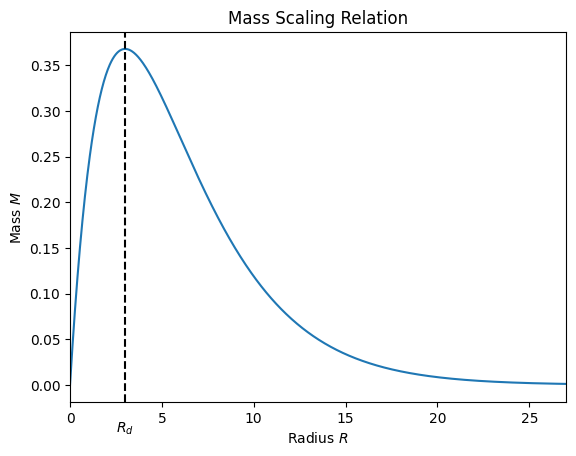
\includegraphics[width=0.8\textwidth]{resources/ring_mass_scaling.png}
        \caption{The mass scaling function from \( R = 0 \) to \( R=27 \) with \( M_d = 1 \) and \( R_d = 3 \).}\label{fig:ring_mass}
    \end{center}
\end{figure}

We now want to explore how this mass scaling affects the scaling of the inertia tensor components to see if there are different
regimes.

\subsection{Inertia Tensor Components Scaling Relations}
Recall that the inertia tensor components are
\begin{align*}
    I_{xx} & = M
    \left[
        \frac{K\left(-{e'}^{2}\right) -\left(1 - e^2\right)E\left(-{e'}^{2}\right)}{e^2K\left(e^2\right)}
        \right]
    ab R^2                                                           \\
    I_{yy} & = M
    \left[
        \frac{E\left(-{e'}^{2}\right) - K\left(-{e'}^{2}\right)}{e^2K\left(e^2\right)}
        \right]
    ab R^2                                                           \\
    I_{zz} & = M \frac{E\left(e^2\right)}{K\left(e^2\right)} a^2 R^2
\end{align*}
and notice that the components are proportional to the quantity
\begin{equation}
    I_{\alpha\alpha} \propto M(R)R^2 \label{eq:inertia_mass_radius_scaling}
\end{equation}
where \( \alpha \in \left\{ x, y, z \right\} \), as we have imposed that the mass is a function of radius, but the %chktex 21
other terms such as the eccentricity and semi-minor and major axes scale lengths are constant. Substituting
Eqn.~\ref{eq:ring_mass} into Eqn.~\ref{eq:inertia_mass_radius_scaling} gives us the pure radius scaling relation of the inertia
tensor components
\begin{align}
    I_{\alpha\alpha}          & \propto \frac{M_{d}R}{R_d} \exp\left(-\frac{R}{R_d}\right) R^2 \nonumber      \\
                              & \propto \frac{M_{d}R^3}{R_d} \exp\left(-\frac{R}{R_d}\right) \nonumber        \\
    \implies I_{\alpha\alpha} & \propto R^3 \exp\left(-\frac{R}{R_d}\right) \label{eq:inertia_radius_scaling}
\end{align}
Differentiating this with respect to \( R \) gives us the stationary points of the scaling relation,
\begin{equation}
    \dbyd{I_{\alpha\alpha}}{R}= C\left[3R^2 \exp\left(-\frac{R}{R_d}\right) - \frac{R^3}{R_d} \exp\left(-\frac{R}{R_d}\right)\right]
\end{equation}
where \( C \) is the proportionality constant. Setting this to zero and solving for \( R \) gives us the stationary points
\begin{align}
    0             & = C\left[3R^2 \exp\left(-\frac{R}{R_d}\right) - \frac{R^3}{R_d} \exp\left(-\frac{R}{R_d}\right)\right] \nonumber \\
                  & = 3R^2 - \frac{R^3}{R_d} \nonumber                                                                               \\
                  & = 3 - \frac{R}{R_d} \nonumber                                                                                    \\
    \frac{R}{R_d} & = 3 \nonumber                                                                                                    \\
    \implies R    & = 3R_d
\end{align}
hence there is a stationary point at \( R = 3R_d \). The second derivative of the inertia tensor components will then help
determine whether this point is a maximum, minimum or a saddle point.
% NOTE: Not bothered to write the derivation of the second derivative
\begin{equation}
    \frac{d^2I_{\alpha\alpha}}{dR^2} = CR\frac{6R_d^2 - 6R_d R + R^2}{R_d^2} \exp\left(-R/R_d\right)
\end{equation}
Evaluating at \( R = 3R_d \) gives the value
\begin{equation}
    \frac{d^2I_{\alpha\alpha}}{dR^2} = -9CR_d\exp(-3) < 0
\end{equation}
and so the point \( R=3R_d \) is a maximum. This is clear when looking at its plot in Fig.~\ref{fig:inertia_radius_scaling}.

\begin{figure}
    \begin{center}
        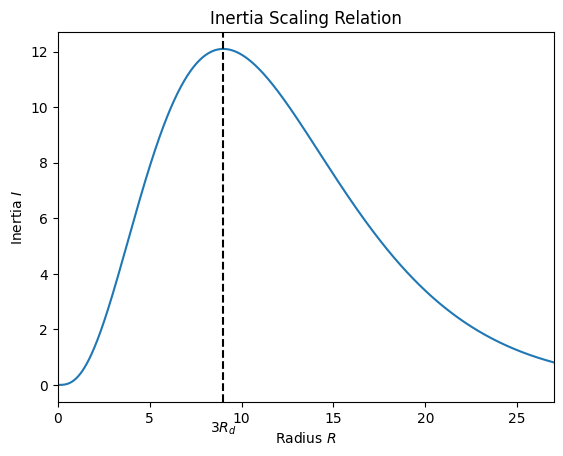
\includegraphics[width=0.8\textwidth]{resources/ring_inertia_scaling.png}
        \caption{The inertia tensor components scaling function from \( R = 0 \) to \( R=27 \) with \( M_d = 1 \) and \( R_d = 3 \).}\label{fig:inertia_radius_scaling}
    \end{center}
\end{figure}

\subsection{Regimes}
Therefore there are three regimes to consider
\begin{enumerate}
    \item{
                \( R < R_d \): The mass and inertia tensor components are both increasing with radius.
          }
    \item{
                \( R_d < R < 3R_d \): The mass is decreasing with radius but the inertia tensor components are increasing.
          }
    \item{
                \( R > 3R_d \): The mass and inertia tensor components are both decreasing with radius.
          }
\end{enumerate}
Hence we will run simulations for these three regimes. An issue to consider when setting the disk scale length parameter \( R_d \)
is the problem of rings bunching up together. If the rings are separated by a small amount in radius, there can be regions
where the density is very large which causes extreme torques. This leads to numerical instability with the current scheme and
so to limit the effect we must use a large disk scale length.

\end{document}
